\documentclass{article}

\usepackage{graphicx}
\usepackage{tikz}
\usepackage{tikzsymbols}
\usetikzlibrary{calc,patterns,shapes.geometric}
\pagestyle{empty}
\usepackage[margin=0pt]{geometry}
\geometry{papersize={14in,12in}}

\def\centerarc[#1](#2)(#3:#4:#5){\draw[#1] ($(#2)+({#5*cos(#3)},{#5*sin(#3)})$) arc (#3:#4:#5);}

\begin{document}
	\begin{figure}
		\centering
		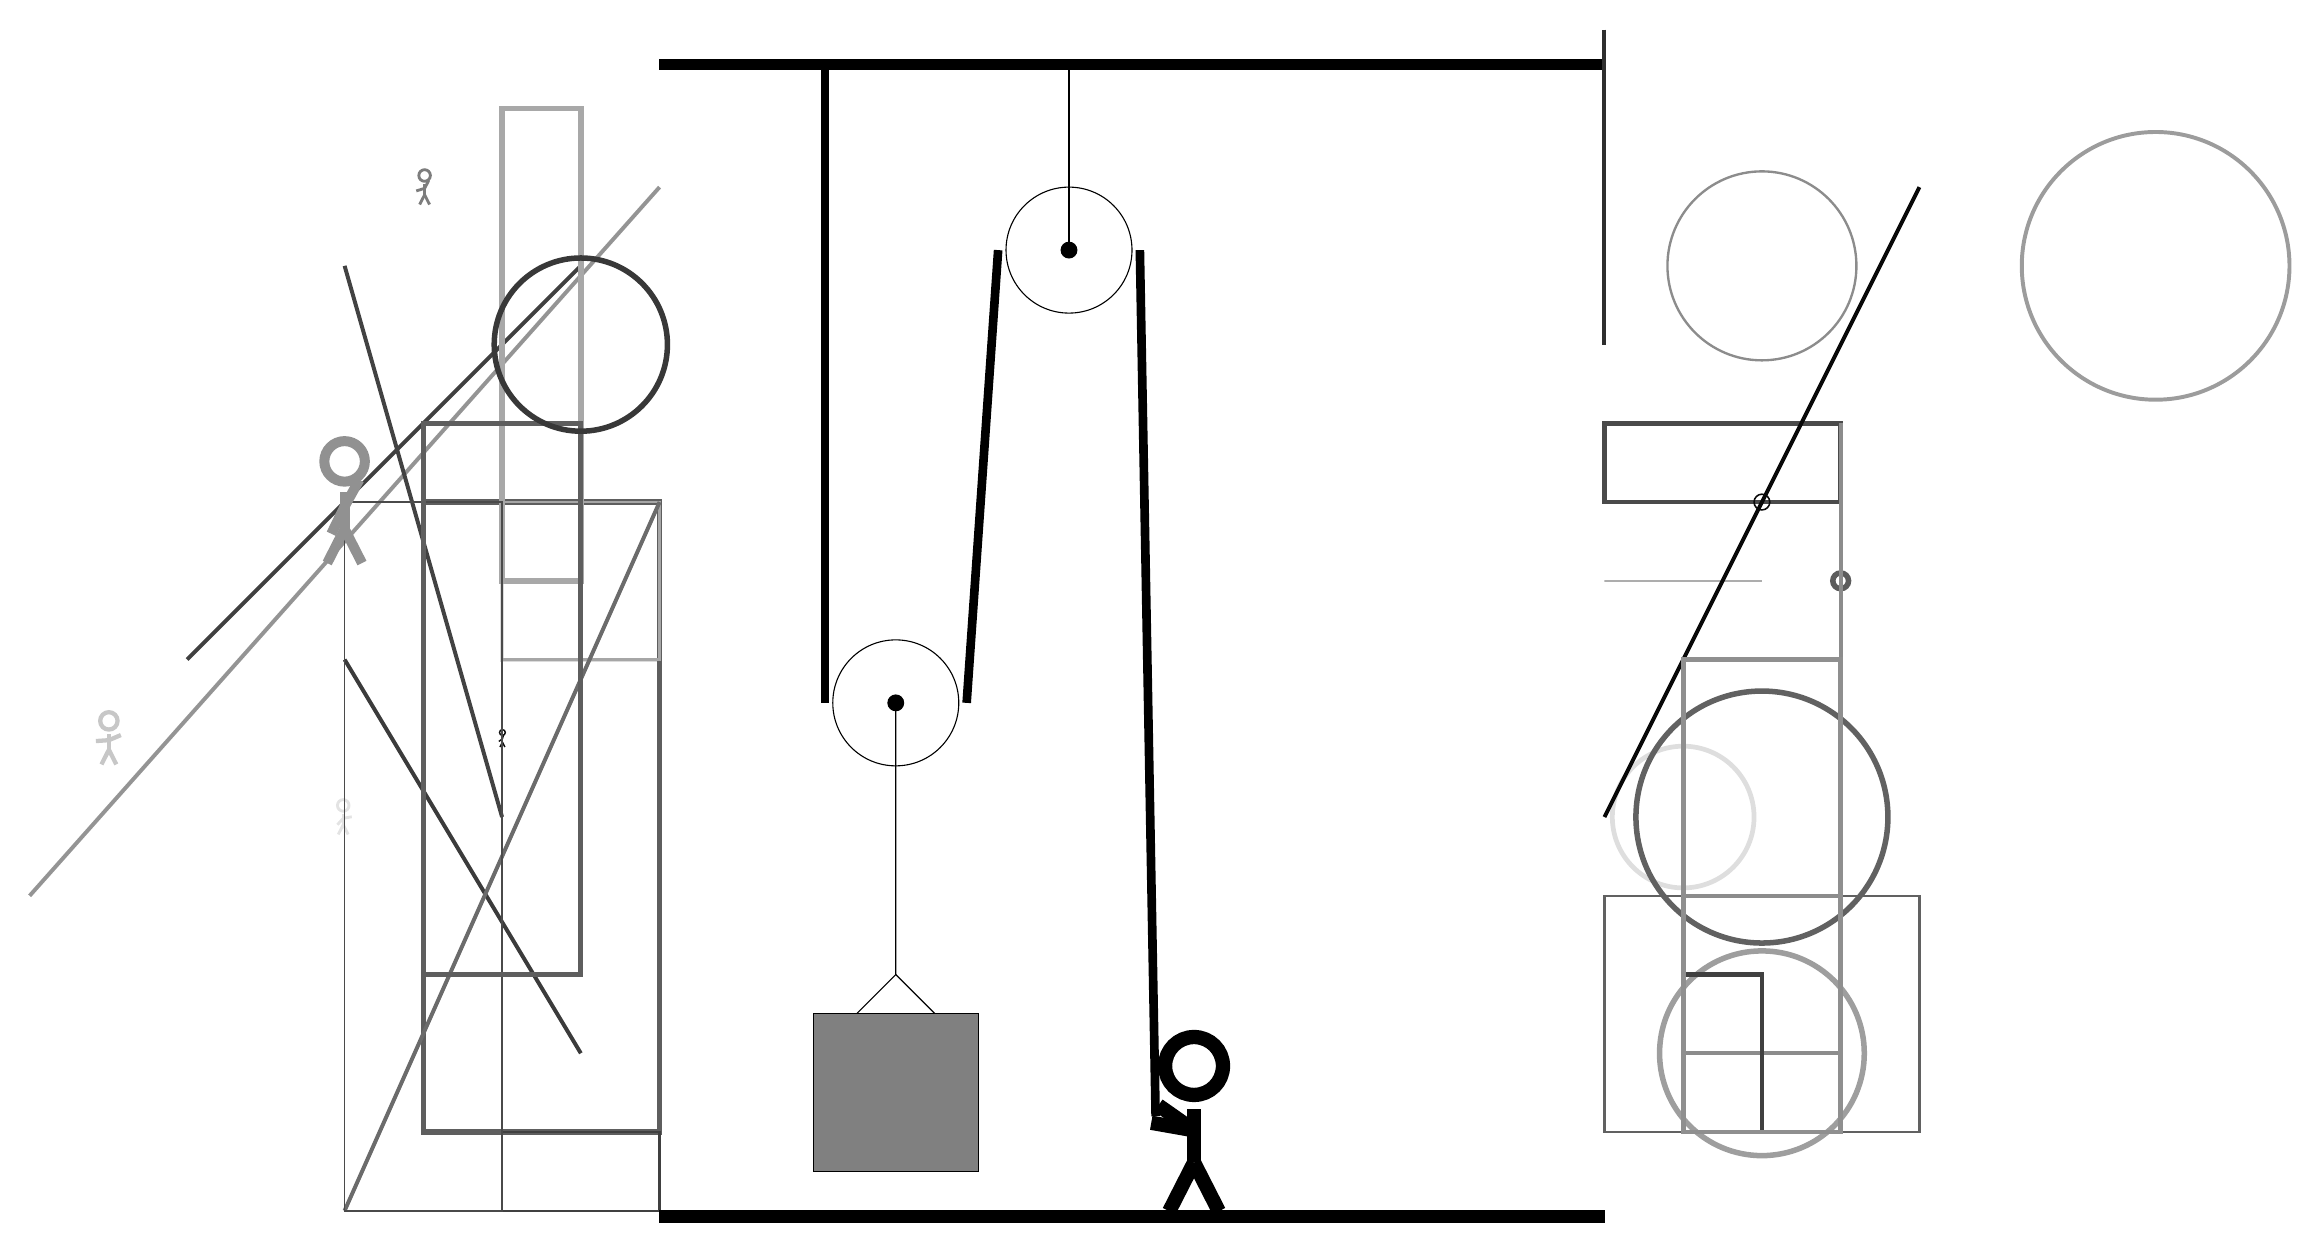
\begin{tikzpicture}
			%%%%% START %%%%%
			
			\draw[fill=black] (-2, 11.5) rectangle (10, 11.625);
			
			\draw [line width=0.7mm, color=black!64](13, 5) circle (0.1);
			
			\draw [line width=0.5mm, color=black!39](17, 9) circle (1.7);
			\draw[line width=0.5mm, color=black!42](-2, 10) -- (-10, 1);
			\draw[line width=0.3mm, color=black!62] (10, 1) rectangle (14, -2);
			\draw[line width=0.5mm, color=black!14] (-4, 6) rectangle (-2, 4);
			\draw [line width=0.7mm, color=black!38](12, -1) circle (1.3);
			\draw[line width=0.7mm, color=black!63] (-2, 6) rectangle (-5, -2);
			
			\draw[line width=0.5mm, color=black!75](-3, 9) -- (-8, 4);
			\node[line width=0.4mm, color=black!51] at (-5, 10) {\Strichmaxerl[2][17][62]};
			\node[line width=0.6mm, color=black!11] at (-6, 2) {\Strichmaxerl[2][48][10]};
			\draw [line width=0.3mm, color=black!45](12, 9) circle (1.2);
			
			\draw[line width=0.3mm, color=black!35] (-2, 6) rectangle (-4, 4);
			\draw[line width=0.5mm, color=black!45] (11, 1) rectangle (13, -1);
			
			\draw[line width=0.7mm, color=black!34] (-4, 5) rectangle (-3, 11);
			\draw[line width=0.5mm, color=black!77](-6, 4) -- (-3, -1);
			\node[line width=0.4mm, color=black!95] at (-4, 3) {\Strichmaxerl[1][35][74]};
			\draw[line width=0.5mm, color=black!74](-4, 2) -- (-6, 9);
			\draw[line width=0.3mm, color=black!75] (-4, -2) rectangle (-2, -3);
			\draw [line width=0.6mm, color=black!13](11, 2) circle (0.9);
			
			\draw[line width=0.6mm, color=black!75] (12, -2) rectangle (11, 0);
			\draw[line width=0.5mm, color=black!58](-2, 6) -- (-6, -3);
			
			\draw[line width=0.2mm, color=black!71] (-4, -3) rectangle (-6, 6);
			
			\draw [line width=0.2mm, color=black!84](-5, -1) circle (0.0);
			\node[line width=0.5mm, color=black!43] at (-6, 6) {\Strichmaxerl[7][64][61]};
			\draw[line width=0.5mm, color=black!45] (12, 4) rectangle (11, 4);
			
			\draw[line width=0.6mm, color=black!71] (10, 7) rectangle (13, 6);
			\draw[line width=0.6mm, color=black!63] (-3, 7) rectangle (-5, 0);
			\draw [line width=0.7mm, color=black!62](12, 2) circle (1.6);
			
			\draw[line width=0.2mm, color=black!32] (12, 5) rectangle (10, 5);
			\draw[line width=0.5mm, color=black!45](13, -2) -- (13, 7);
			\draw[line width=0.5mm, color=black!97](10, 2) -- (14, 10);
			\draw[line width=0.6mm, color=black!44] (11, 4) rectangle (13, -2);
			\draw[line width=0.5mm, color=black!82](10, 12) -- (10, 8);
			\draw [line width=0.7mm, color=black!78](-3, 8) circle (1.1);
			\draw [line width=0.2mm, color=black!96](12, 6) circle (0.1);
			\node[line width=0.5mm, color=black!22] at (-9, 3) {\Strichmaxerl[3][4][23]};
			
			\draw (3.2, 9.2) circle (0.8);
			\draw[fill=black] (3.2, 9.2) circle (0.1);
			\draw[thick] (3.2, 9.2) -- (3.2, 11.5);
			
			\draw (1, 3.45) circle (0.8);
			\draw[fill=black] (1, 3.45) circle (0.1);
			
			\draw (1, 3.45) -- (1, 0.0) -- (0.5, -0.5);
			\draw (1, 0.0) -- (1.5, -0.5);
			\draw[fill=black!50] (-0.05, -0.5) rectangle (2.05, -2.5);
			
			\draw[line width=1.1mm] (0.1, 11.5) -- (0.1, 3.45);
			\centerarc[line width=1.1mm](1, 3.45)(180:360:0.9);
			\draw[line width=1.1mm](1.9, 3.45) -- (2.3, 9.2);
			\centerarc[line width=1.1mm](3.2, 9.2)(0:180:0.9);
			\draw[line width=1.1mm](4.1, 9.2) -- (4.3, -1.8);
			
			\node at (4.7, -1.9) {\Strichmaxerl[10][-35][170]};
			
			\draw[fill=black] (-2, -3) rectangle (10, -3.15);
			
			%%%%% END %%%%%
		\end{tikzpicture}
	\end{figure}	
\end{document}